% setwd('C:/aaaWork/Class Materials/MTH207/Year_Specific/W11/Assessments/')
% Sweave("Quiz2_Results.Rnw",stylepath=TRUE)

\documentclass[a4paper]{article}
\input{c:/aaaWork/zGnrlLatex/GnrlPreamble}

\usepackage{C:/Apps/R-2.12.1/share/texmf/tex/latex/Sweave}
\begin{document}


\title{Quiz 2 Handout}
\date{}  % makes date blank -- title will only have the title above then
\maketitle
\vspace{-36pt}


\vspace{-36pt}
\section*{Background}
Sanz (2001)  examined the nesting behavior and success for male and female pied flycatchers (\textit{Ficedula hypoleuca}).  He hypothesized that males would be more involved in nesting activities as the level of brood demand increased and as the ``attractiveness'' of the male decreased.  The author manipulated brood demand by removing two eggs from randomly selected nests and placing these eggs into other randomly selected nests.  This created two levels for a ``clutch-size manipulation'' factor - reduced and enlarged clutch sizes.  A third level consisted of nests where the number of eggs was not manipulated (called the ``control'' level).  The author manipulated the ``attractiveness'' of the male by reducing the size of the white patch on the forehead.  The forehead patch was reduced in size on randomly selected males by clipping approximately two-thirds of the white feathers.  Thus, the experiment consisted of two levels of the ``forehead patch'' factor - ``unmanipulated'' and ``reduced.''  In one aspect of the experiment, Sanz recorded the feeding rate of the male flycatchers on the 13th day post-hatch.  The feeding rate was recorded as the number of times the male fed the hatchlings per hour.  The author tested his hypotheses by examining the data for clutch-size manipulation (\var{csm}), forehead manipulation (\var{fh}), and interaction effects on feeding rates (\var{mfr}).

\section*{R Results}
\begin{Schunk}
\begin{Sinput}
> library(NCStats)
> library(multcomp)
\end{Sinput}
\end{Schunk}

\vspace{-18pt}

\begin{Schunk}
\begin{Sinput}
> pfc <- read.table("PiedFlycatcher1.txt",head=TRUE)
> str(pfc)
\end{Sinput}
\begin{Soutput}
'data.frame':	74 obs. of  3 variables:
 $ csm: Factor w/ 3 levels "control","enlarged",..: 1 1 1 1 1 1 1 1 1 1 ...
 $ fh : Factor w/ 2 levels "reduced","unmanip": 2 2 2 2 2 2 2 2 2 2 ...
 $ mfr: int  0 13 11 3 24 12 26 36 17 19 ...
\end{Soutput}
\begin{Sinput}
> pfc$csm <- factor(pfc$csm,levels=c("reduced","control","enlarged"))
> lm1 <- lm(mfr~csm*fh,data=pfc)
> leveneTest(lm1)
\end{Sinput}
\begin{Soutput}
Levene's Test for Homogeneity of Variance (center = median)
      Df F value Pr(>F)
group  5  0.8643 0.5097
      68               
\end{Soutput}
\begin{Sinput}
> adTest(lm1$residuals)
\end{Sinput}
\begin{Soutput}
	Anderson-Darling normality test

data:  lm1$residuals 
A = 0.261, p-value = 0.6989
\end{Soutput}
\begin{Sinput}
> outlierTest(lm1)
\end{Sinput}
\begin{Soutput}
No Studentized residuals with Bonferonni p < 0.05
Largest |rstudent|:
   rstudent unadjusted p-value Bonferonni p
24 2.461379           0.016422           NA
\end{Soutput}
\begin{Sinput}
> hist(lm1$residuals,main="",xlab="Residuals")
> residualPlot(lm1,main="")
\end{Sinput}
\end{Schunk}
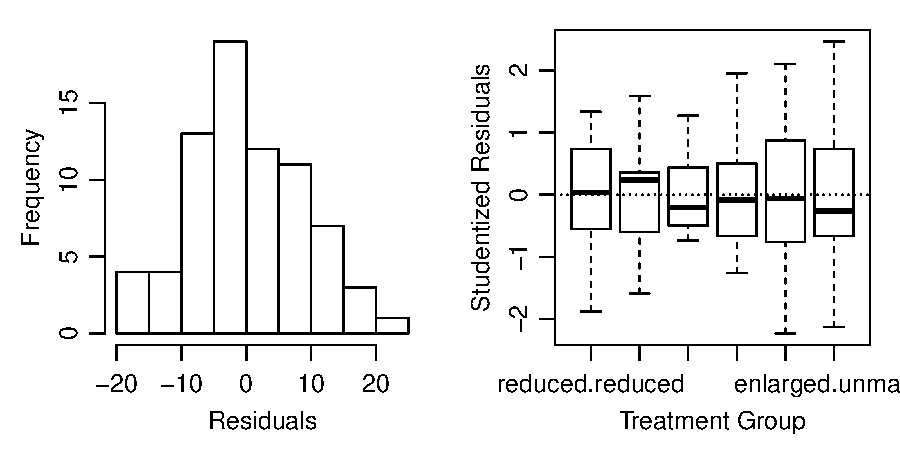
\includegraphics[width=4.5in]{Figs/q2-untrResids.PDF}

\begin{Schunk}
\begin{Sinput}
> anova(lm1)
\end{Sinput}
\end{Schunk}
\begin{Schunk}
\begin{Soutput}
          Df Sum Sq Mean Sq F value  Pr(>F)
csm        2  750.9  375.44  4.7771 0.01145
fh         1  315.9  315.88  4.0193 0.04897
csm:fh     2   77.0   38.48  0.4896 0.61503
Residuals 68 5344.1   78.59                
\end{Soutput}
\end{Schunk}


\begin{Schunk}
\begin{Sinput}
> fitPlot(lm1,legend="topleft",ylim=c(9,26),main="",interval=FALSE)
> fitPlot(lm1,which="csm",ylim=c(9,26),main="")
> fitPlot(lm1,which="fh",ylim=c(9,26),main="")
\end{Sinput}
\end{Schunk}
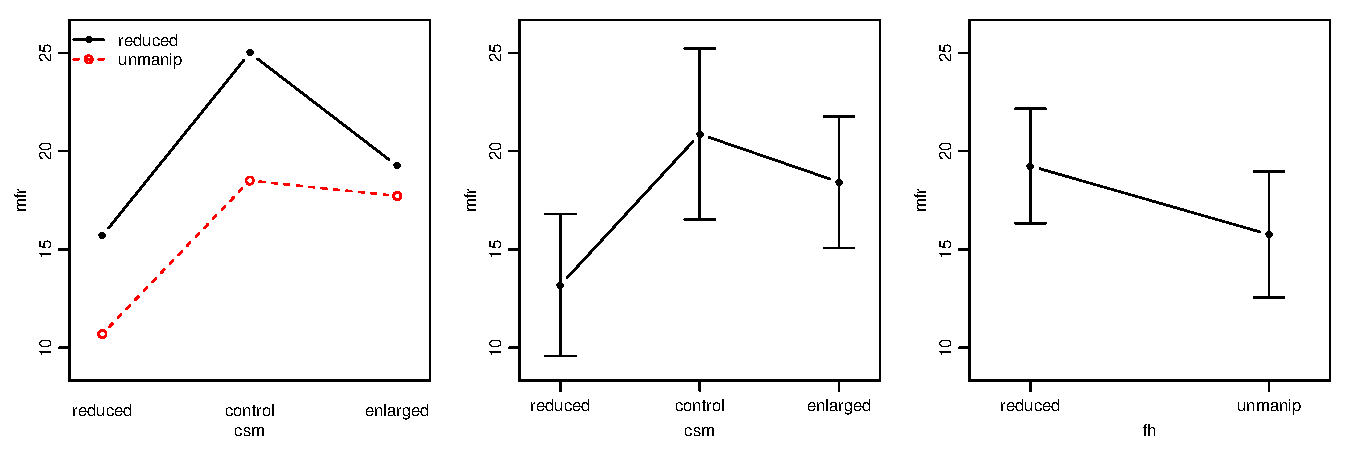
\includegraphics[width=7in]{Figs/q2-untrFits.PDF}

\begin{Schunk}
\begin{Sinput}
> mc1 <- glht(lm1,mcp(csm="Tukey"))
> summary(mc1)
\end{Sinput}
\end{Schunk}
\begin{Schunk}
\begin{Soutput}
                        Estimate Std. Error   t value     p value
control - reduced = 0   8.241742   2.564876  3.213310 0.005475138
enlarged - reduced = 0  5.391655   2.442048  2.207842 0.076664737
enlarged - control = 0 -2.850087   2.557330 -1.114478 0.508294723
\end{Soutput}
\end{Schunk}
\begin{Schunk}
\begin{Sinput}
> pfc$comb <- pfc$csm:pfc$fh
> lm1a <- lm(mfr~comb,data=pfc)
> mc1a <- glht(lm1a,mcp(comb="Tukey"))
> summary(mc1a)
\end{Sinput}
\end{Schunk}
\begin{Schunk}
\begin{Soutput}
                                          Estimate Std. Error    t value     p value
reduced:unmanip - reduced:reduced = 0   -5.0000000   3.477187 -1.4379441 0.702573150
control:reduced - reduced:reduced = 0    9.3076923   3.983618  2.3364923 0.192779682
control:unmanip - reduced:reduced = 0    2.8076923   3.414530  0.8222779 0.962144218
enlarged:reduced - reduced:reduced = 0   3.5576923   3.548889  1.0024806 0.914997266
enlarged:unmanip - reduced:reduced = 0   2.0219780   3.414530  0.5921688 0.991168825
control:reduced - reduced:unmanip = 0   14.3076923   3.983618  3.5916328 0.007796999
control:unmanip - reduced:unmanip = 0    7.8076923   3.414530  2.2866085 0.212569829
enlarged:reduced - reduced:unmanip = 0   8.5576923   3.548889  2.4113724 0.165799466
enlarged:unmanip - reduced:unmanip = 0   7.0219780   3.414530  2.0564994 0.320874928
control:unmanip - control:reduced = 0   -6.5000000   3.929045 -1.6543460 0.564443257
enlarged:reduced - control:reduced = 0  -5.7500000   4.046356 -1.4210317 0.712914972
enlarged:unmanip - control:reduced = 0  -7.2857143   3.929045 -1.8543219 0.437172894
enlarged:reduced - control:unmanip = 0   0.7500000   3.487520  0.2150525 0.999933257
enlarged:unmanip - control:unmanip = 0  -0.7857143   3.350701 -0.2344925 0.999897684
enlarged:unmanip - enlarged:reduced = 0 -1.5357143   3.487520 -0.4403456 0.997798702
\end{Soutput}
\end{Schunk}

\begin{Schunk}
\begin{Sinput}
> pfc$logmfr <- log(pfc$mfr+0.01)
> lm2 <- lm(logmfr~csm*fh,data=pfc)
> leveneTest(lm2)
\end{Sinput}
\begin{Soutput}
Levene's Test for Homogeneity of Variance (center = median)
      Df F value Pr(>F)
group  5  0.9781 0.4376
      68               
\end{Soutput}
\begin{Sinput}
> adTest(lm2$residuals)
\end{Sinput}
\begin{Soutput}
	Anderson-Darling normality test

data:  lm2$residuals 
A = 9.7963, p-value < 2.2e-16
\end{Soutput}
\begin{Sinput}
> hist(lm2$residuals,main="")
> residualPlot(lm2,main="")
\end{Sinput}
\end{Schunk}
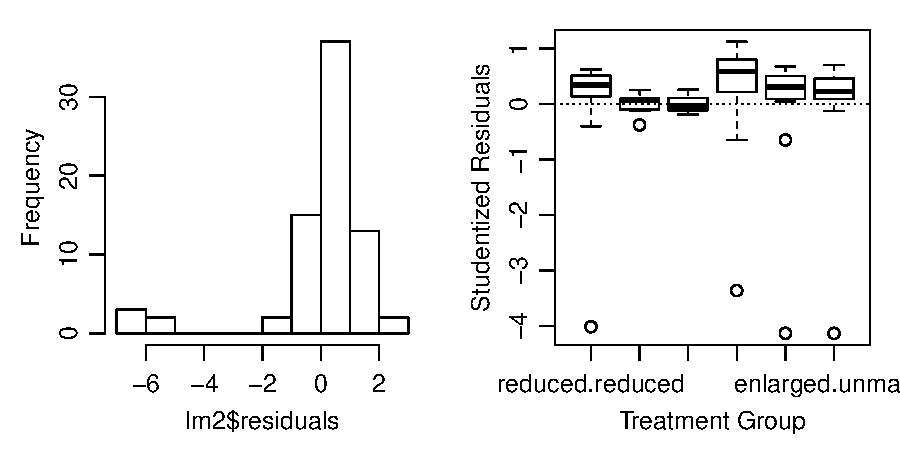
\includegraphics[width=4.5in]{Figs/q2-trResids.PDF}

\begin{Schunk}
\begin{Sinput}
> anova(lm2)
\end{Sinput}
\end{Schunk}
\begin{Schunk}
\begin{Soutput}
          Df  Sum Sq Mean Sq F value  Pr(>F)
csm        2  14.739  7.3694  1.9733 0.14688
fh         1  11.229 11.2289  3.0067 0.08745
csm:fh     2   0.371  0.1857  0.0497 0.95153
Residuals 68 253.951  3.7346                
\end{Soutput}
\end{Schunk}


\begin{Schunk}
\begin{Sinput}
> fitPlot(lm2,legend="topleft",ylim=c(1.2,3.4),main="",interval=FALSE)
> fitPlot(lm2,which="csm",ylim=c(1.2,3.4),main="")
> fitPlot(lm2,which="fh",ylim=c(1.2,3.4),main="")
\end{Sinput}
\end{Schunk}
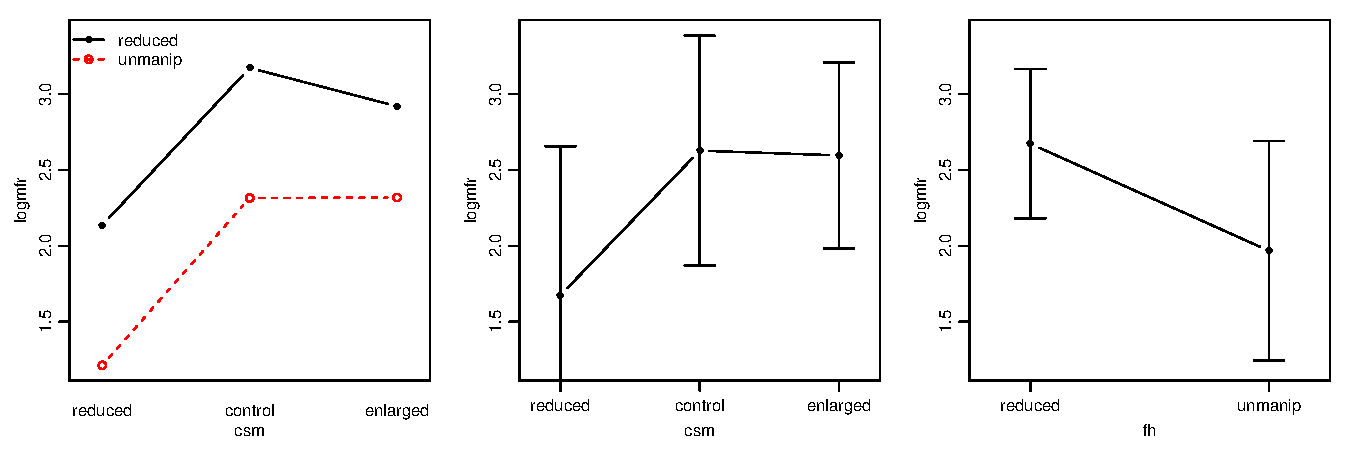
\includegraphics[width=7in]{Figs/q2-trFits.PDF}

\begin{Schunk}
\begin{Sinput}
> mc2a <- glht(lm2,mcp(csm="Tukey"))
> summary(mc2a)
\end{Sinput}
\end{Schunk}
\begin{Schunk}
\begin{Soutput}
                         Estimate Std. Error    t value   p value
control - reduced = 0   1.0344433  0.8683878  1.1912227 0.4615795
enlarged - reduced = 0  0.7813633  0.7736213  1.0100075 0.5723424
enlarged - control = 0 -0.2530799  0.8820640 -0.2869179 0.9555398
\end{Soutput}
\end{Schunk}
\begin{Schunk}
\begin{Sinput}
> mc2b <- glht(lm2,mcp(fh="Tukey"))
> summary(mc2b)
\end{Sinput}
\end{Schunk}
\begin{Schunk}
\begin{Soutput}
                        Estimate Std. Error   t value   p value
unmanip - reduced = 0 -0.9235421   0.757991 -1.218408 0.2272795
\end{Soutput}
\end{Schunk}
\begin{Schunk}
\begin{Sinput}
> lm2a <- lm(logmfr~comb,data=pfc)
> mc2c <- glht(lm2a,mcp(comb="Tukey"))
> summary(mc2c)
\end{Sinput}
\end{Schunk}
\begin{Schunk}
\begin{Soutput}
                                            Estimate Std. Error      t value   p value
reduced:unmanip - reduced:reduced = 0   -0.923542109  0.7579910 -1.218407762 0.8254227
control:reduced - reduced:reduced = 0    1.034443253  0.8683878  1.191222727 0.8386153
control:unmanip - reduced:reduced = 0    0.178445506  0.7443324  0.239739009 0.9998859
enlarged:reduced - reduced:reduced = 0   0.781363341  0.7736213  1.010007511 0.9124943
enlarged:unmanip - reduced:reduced = 0   0.181387911  0.7443324  0.243692088 0.9998763
control:reduced - reduced:unmanip = 0    1.957985362  0.8683878  2.254736212 0.2258995
control:unmanip - reduced:unmanip = 0    1.101987615  0.7443324  1.480504741 0.6762910
enlarged:reduced - reduced:unmanip = 0   1.704905450  0.7736213  2.203798437 0.2482281
enlarged:unmanip - reduced:unmanip = 0   1.104930020  0.7443324  1.484457820 0.6736755
control:unmanip - control:reduced = 0   -0.855997747  0.8564915 -0.999423528 0.9160202
enlarged:reduced - control:reduced = 0  -0.253079912  0.8820640 -0.286917852 0.9997238
enlarged:unmanip - control:reduced = 0  -0.853055342  0.8564915 -0.995988112 0.9171282
enlarged:reduced - control:unmanip = 0   0.602917834  0.7602436  0.793058774 0.9675611
enlarged:unmanip - control:unmanip = 0   0.002942405  0.7304184  0.004028383 1.0000000
enlarged:unmanip - enlarged:reduced = 0 -0.599975429  0.7602436 -0.789188429 0.9682227
\end{Soutput}
\end{Schunk}

\end{document}
